\section*{Materiale}

L'attrezzatura utilizzata in questa esperienza di laboratorio e elencata di seguito:

\begin{itemize}
    \setlength{\itemsep}{1pt}
    \item{Breadboard, cavi a banana e cavetti per breadboard;}
    \item{Osilloscopio: Agilent Technologies in grado di distiguere frequenze di massimo $70\,\si{\mega\hertz}$;}
    \item{Generatore di forme d'onde: Agilent Technologies in grado di generare frequenze massime di $15\,\si{\mega\hertz}$;}
    \item{Multimetro (Agilent Technologies) e Oscilloscopio;}
    \item{Resistenze varie;}
    \item{Transistor BC107B, diodo LED;}
    \item{Decadi di resistenze e capacità.}
\end{itemize}

\section*{Circuito}

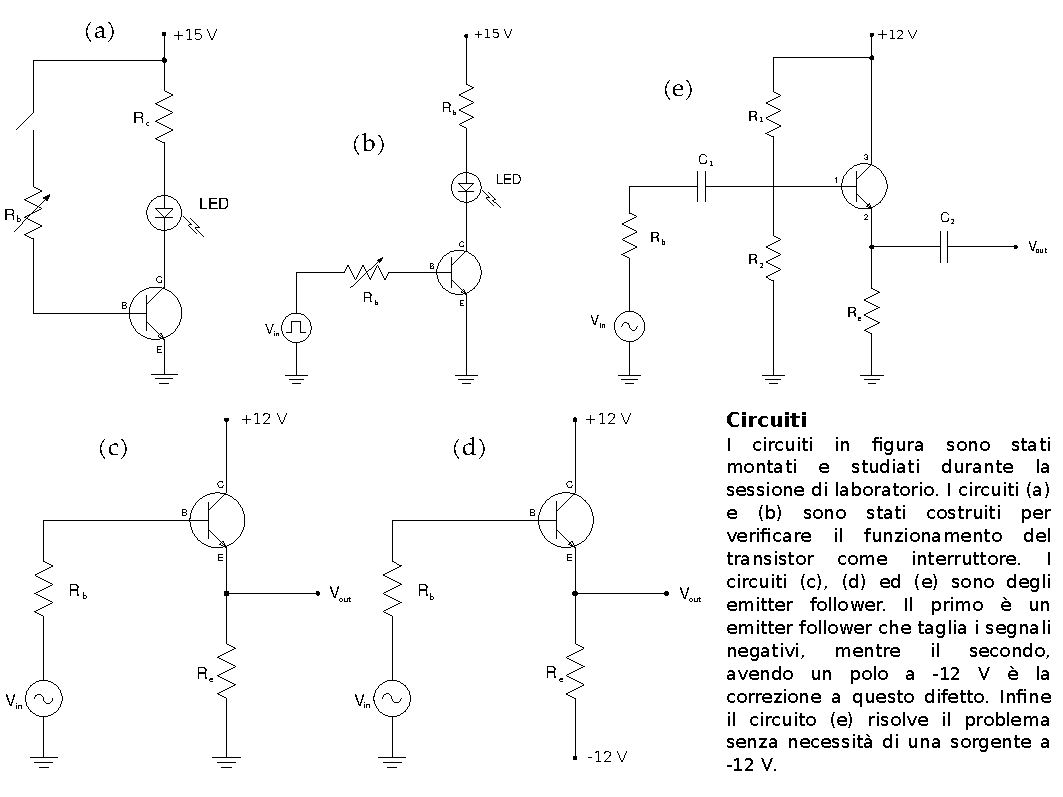
\includegraphics[width=\textwidth]{circuiti.pdf}
